\begin{figure}
	\centering
	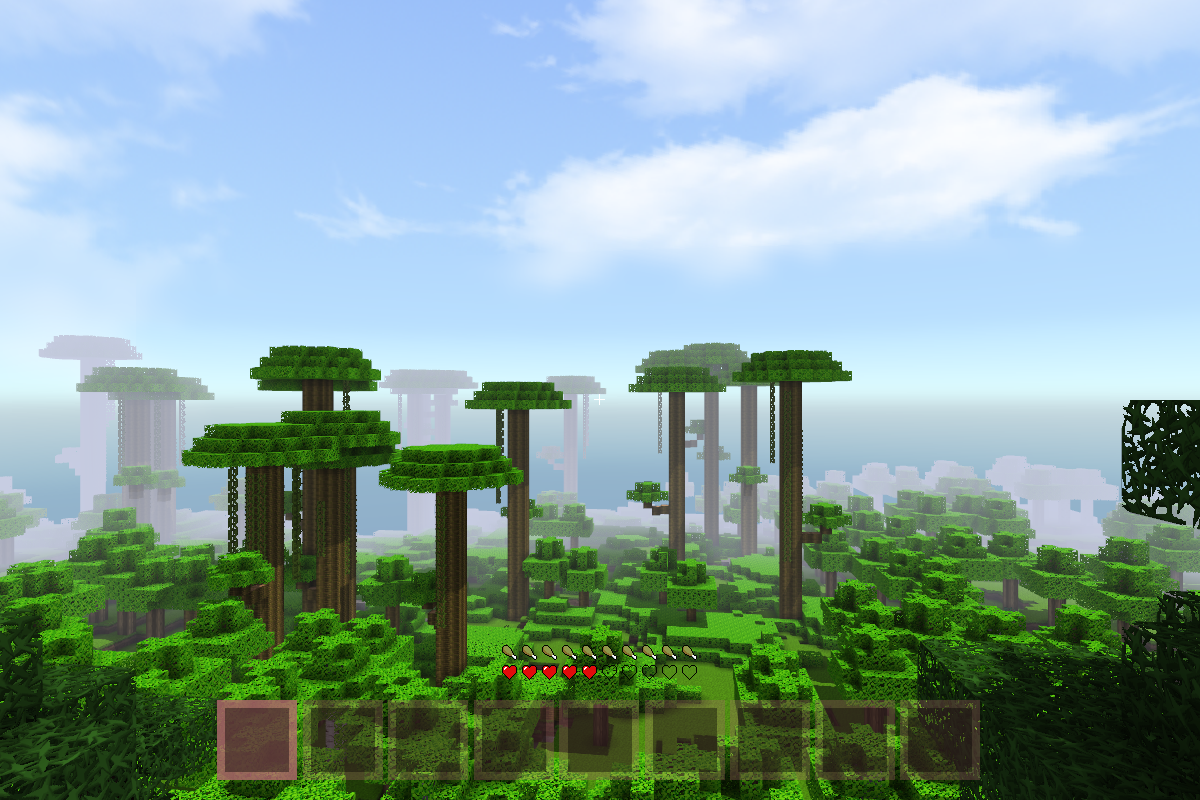
\includegraphics[width=.32\textwidth]{rotate-1.png}
	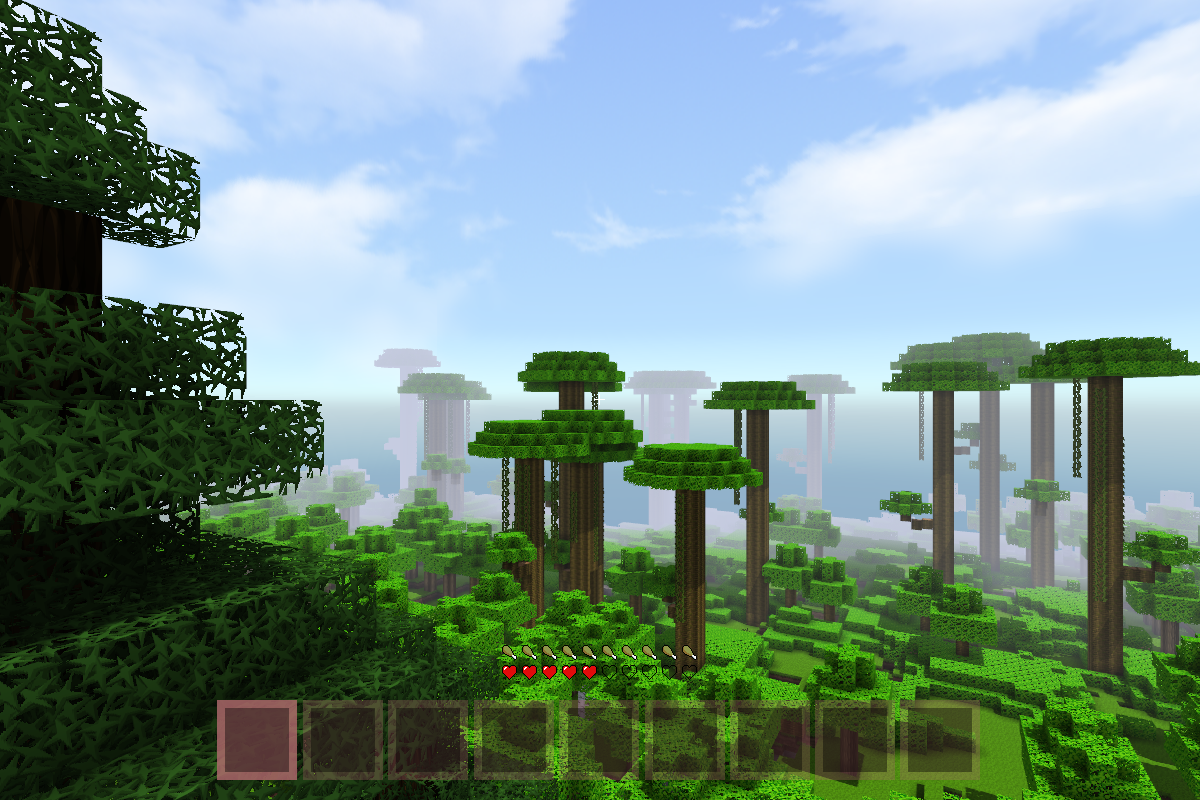
\includegraphics[width=.32\textwidth]{rotate-2.png}
	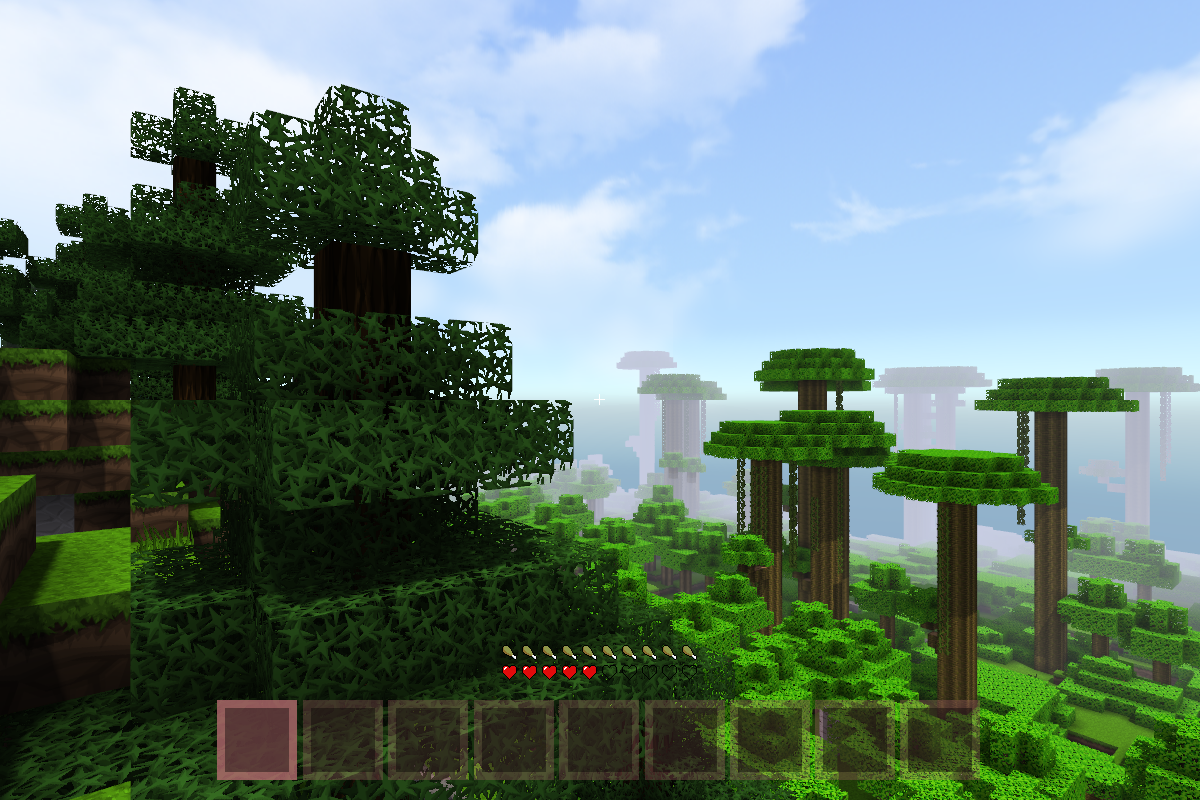
\includegraphics[width=.32\textwidth]{rotate-3.png}\\[4pt]
	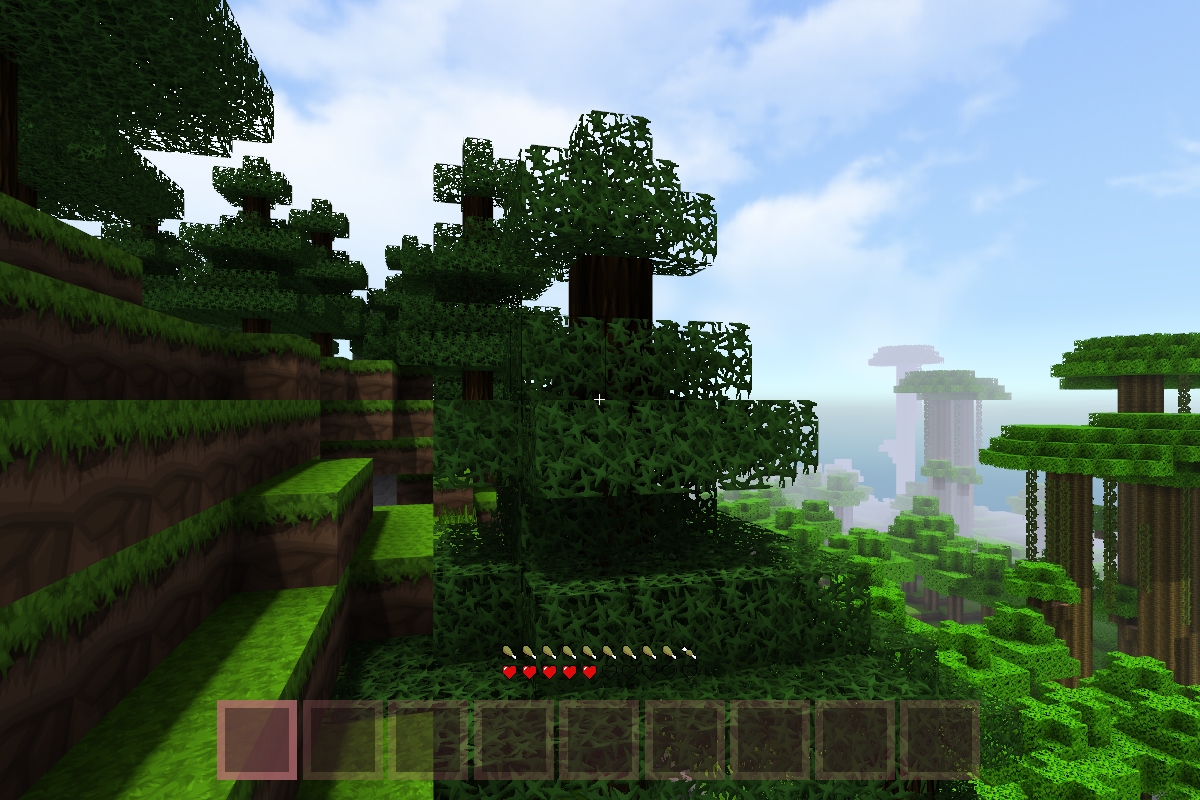
\includegraphics[width=.32\textwidth]{rotate-4.png}
	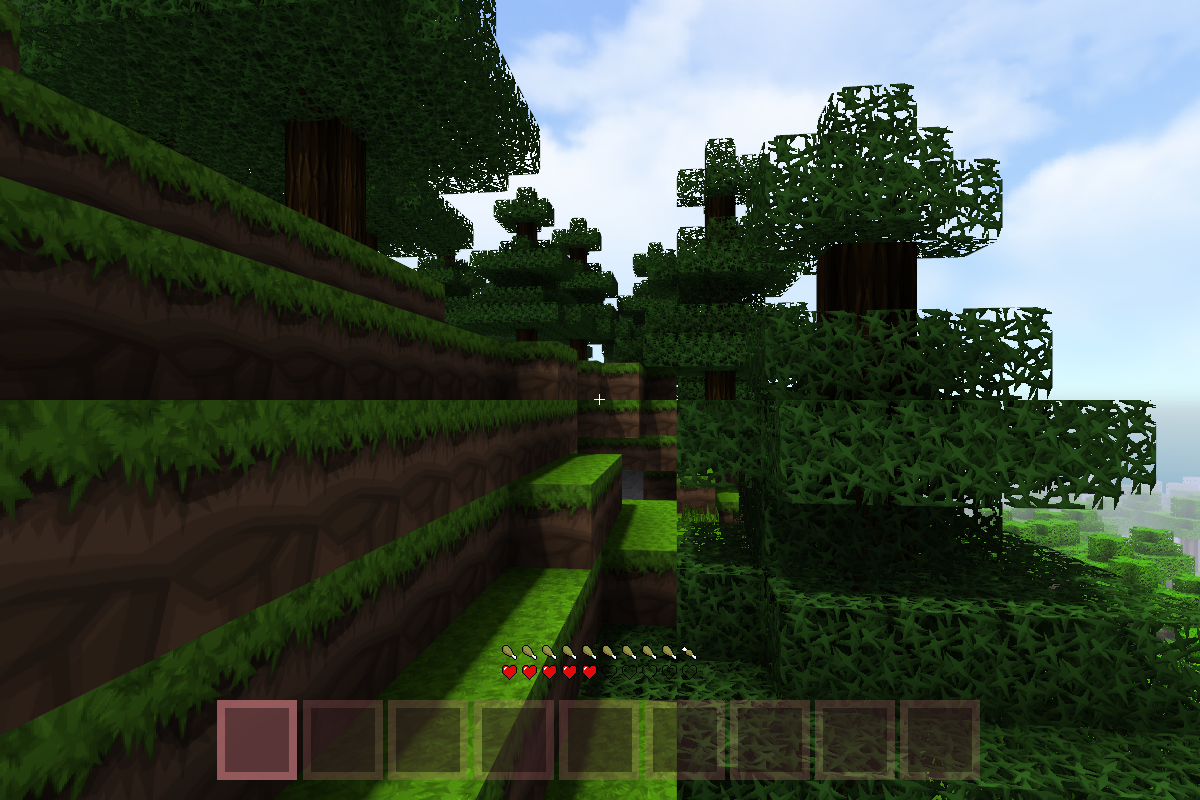
\includegraphics[width=.32\textwidth]{rotate-5.png}
	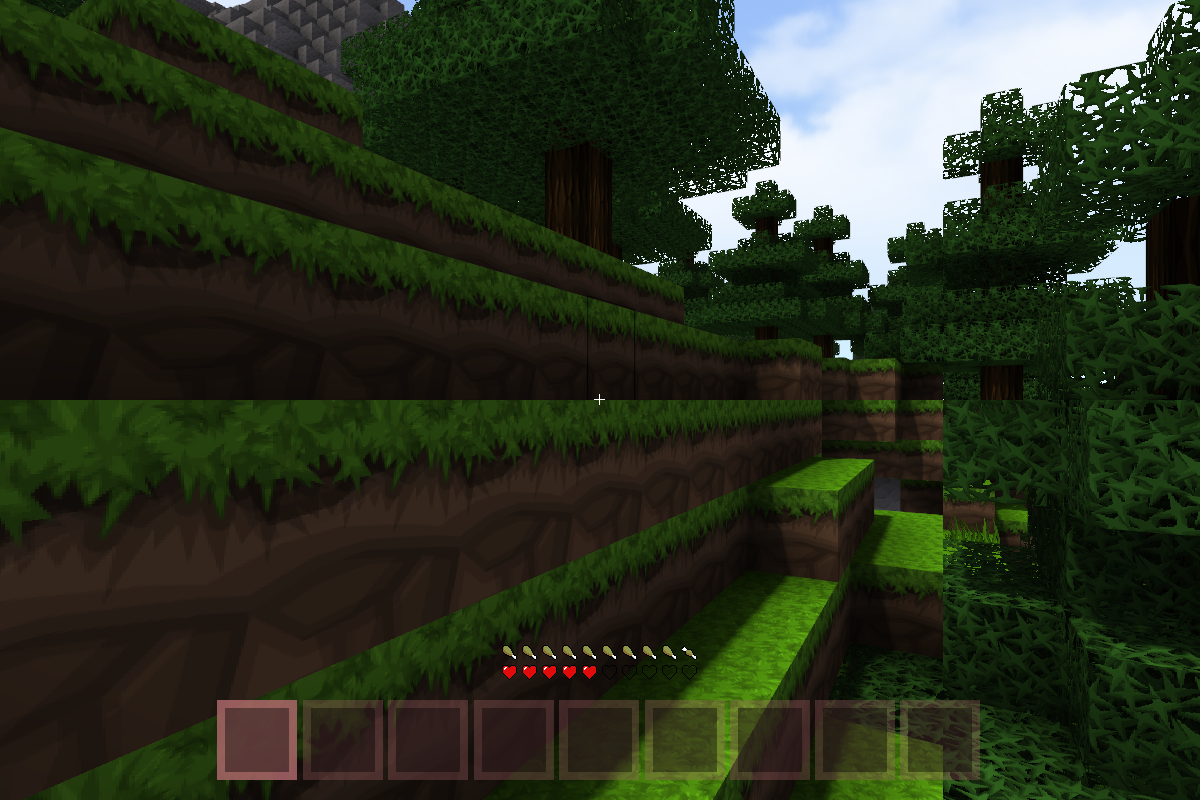
\includegraphics[width=.32\textwidth]{rotate-6.png}
	%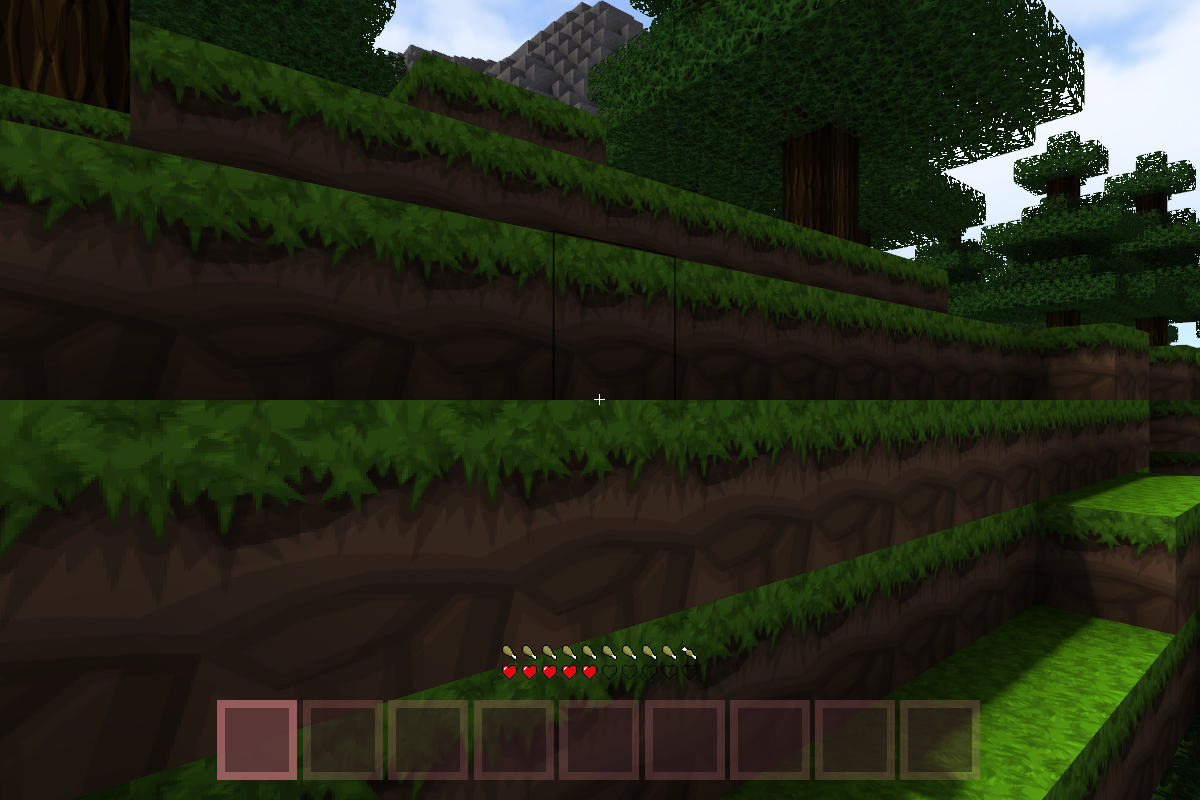
\includegraphics[width=.24\textwidth]{rotate-7.png}
	%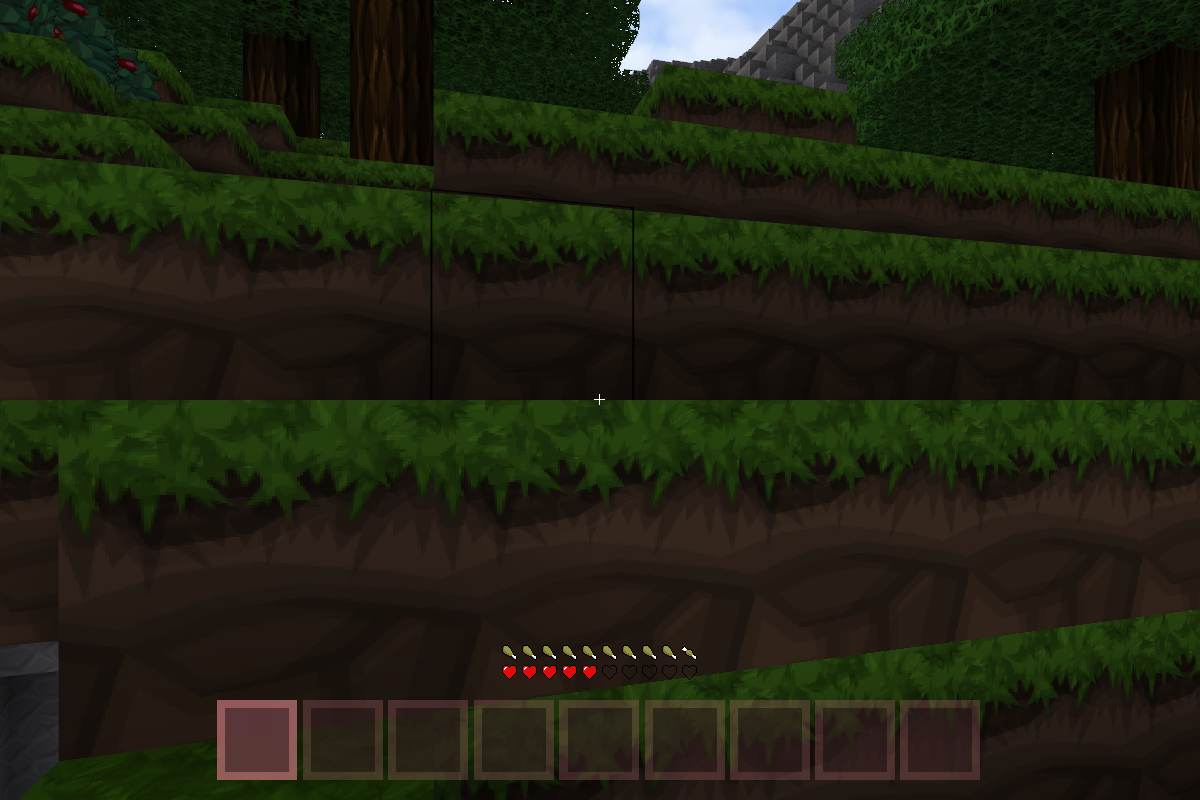
\includegraphics[width=.24\textwidth]{rotate-8.png}
	\caption{t}\label{fig:rotate}
\end{figure}


\begin{figure}[!htbp]
	\fpsplot{seed-0-rotate}
	\caption{Seed 0 Rotation}\label{fig:seed-0-rotate-fps}
\end{figure}

\begin{figure}[!htbp]
	\cpuplot{seed-0-rotate}
	\caption{Seed 0 Rotation}\label{fig:seed-0-rotate-cpu}
\end{figure}

\begin{figure}[!htbp]
	\gpuplot{seed-0-rotate}
	\caption{Seed 0 Rotation}\label{fig:seed-0-rotate-gpu}
\end{figure}

\begin{figure}[!htbp]
	\memplot{seed-0-rotate-single-mem.csv}
	\memplot{seed-0-rotate-multi-mem.csv}
	\caption{Seed 0 Rotation}\label{fig:seed-0-rotate-mem}	
\end{figure} 

